
\chapter{Tracking Examples} \label{Exam}

A simple tracking example is shown with its input file (\ref{input}), its output file (\ref{output}) and some corresponding plots in (\ref{plots}).

% ================================================================================================================================ %
\section{Input Example} \label{input}

For the description of the different input blocks, see Chapters \ref{GenInp} and \ref{SpecElem}.

\begin{ctverbatim}
FREE FORMAT   TITLE: EXAMPLE
PRINTOUT OF INPUT PARAMETERS--------------------------------------------
NEXT--------------------------------------------------------------------
SINGLE ELEMENTS---------------------------------------------------------
    B      0  0.0000000   0.000000  50.00000
    QD2    2  0.0000000   0.009536   0.77000
    QF2    2  0.0000000  -0.009536   0.77000
    MU    11  1.0000000   1.000000   0.00000
    SEX    3  0.0500000   0.000000   0.00000
NEXT--------------------------------------------------------------------
BLOCK DEFINITIONS-------------------------------------------------------
    1  1
    B1  QD2  B  QF2
    B2  QF2  B  QD2
NEXT--------------------------------------------------------------------
STRUCTURE INPUT---------------------------------------------------------
    MU  B1  SEX  B2
NEXT--------------------------------------------------------------------
MULTIPOLE COEFFICIENTS--------------------------------------------------
    MU       10.0       3.5765
    0.0000    0.0000    0.0000    0.0000
    0.0000    0.0000    0.0000    0.0000
    0.405E-3  0.0000    0.0000    0.0000
   -0.5E-5    0.0000    0.0000    0.0000
   -0.56E-4   0.0000    0.0000    0.0000
    0.0000    0.0000    0.0000    0.0000
    0.3E-5    0.0000    0.0000    0.0000
    0.0000    0.0000    0.0000    0.0000
   -0.1E-5    0.0000    0.0000    0.0000
NEXT--------------------------------------------------------------------
TRACKING PARAMETERS-----------------------------------------------------
  10000  0  2  11.0  11.5  0  1
      1  1  0   0
      0  0  1   1  1 50000 2
NEXT--------------------------------------------------------------------
INITIAL COORDINATES-----------------------------------------------------
      2    0.0   0.0   1.0
      0.0
      0.0
      0.0
      0.0
      0.0
      0.0
      0.0
      0.000001
      0.0
      0.0
      0.0
      0.0
 450000.0
 450000.0
 450000.0
NEXT--------------------------------------------------------------------
ITERATION-ACCURACY------------------------------------------------------
    50    1D-14  1D-15
    10    1D-10  1D-10
    10    1D-5   1D-6
    1D-8  1D-12  1D-10
NEXT--------------------------------------------------------------------
POSTPROCESSING----------------------------------------------------------
EXAMPLE
    1000    0    0  1   0.08  0.08   1
       0.0  0.0  1  1  20     0.005  1  0.10
    7878    1    0  1   1     1      1
NEXT
ENDE====================================================================
\end{ctverbatim}

% \begin{figure}[H]
%     \begin{center}
%         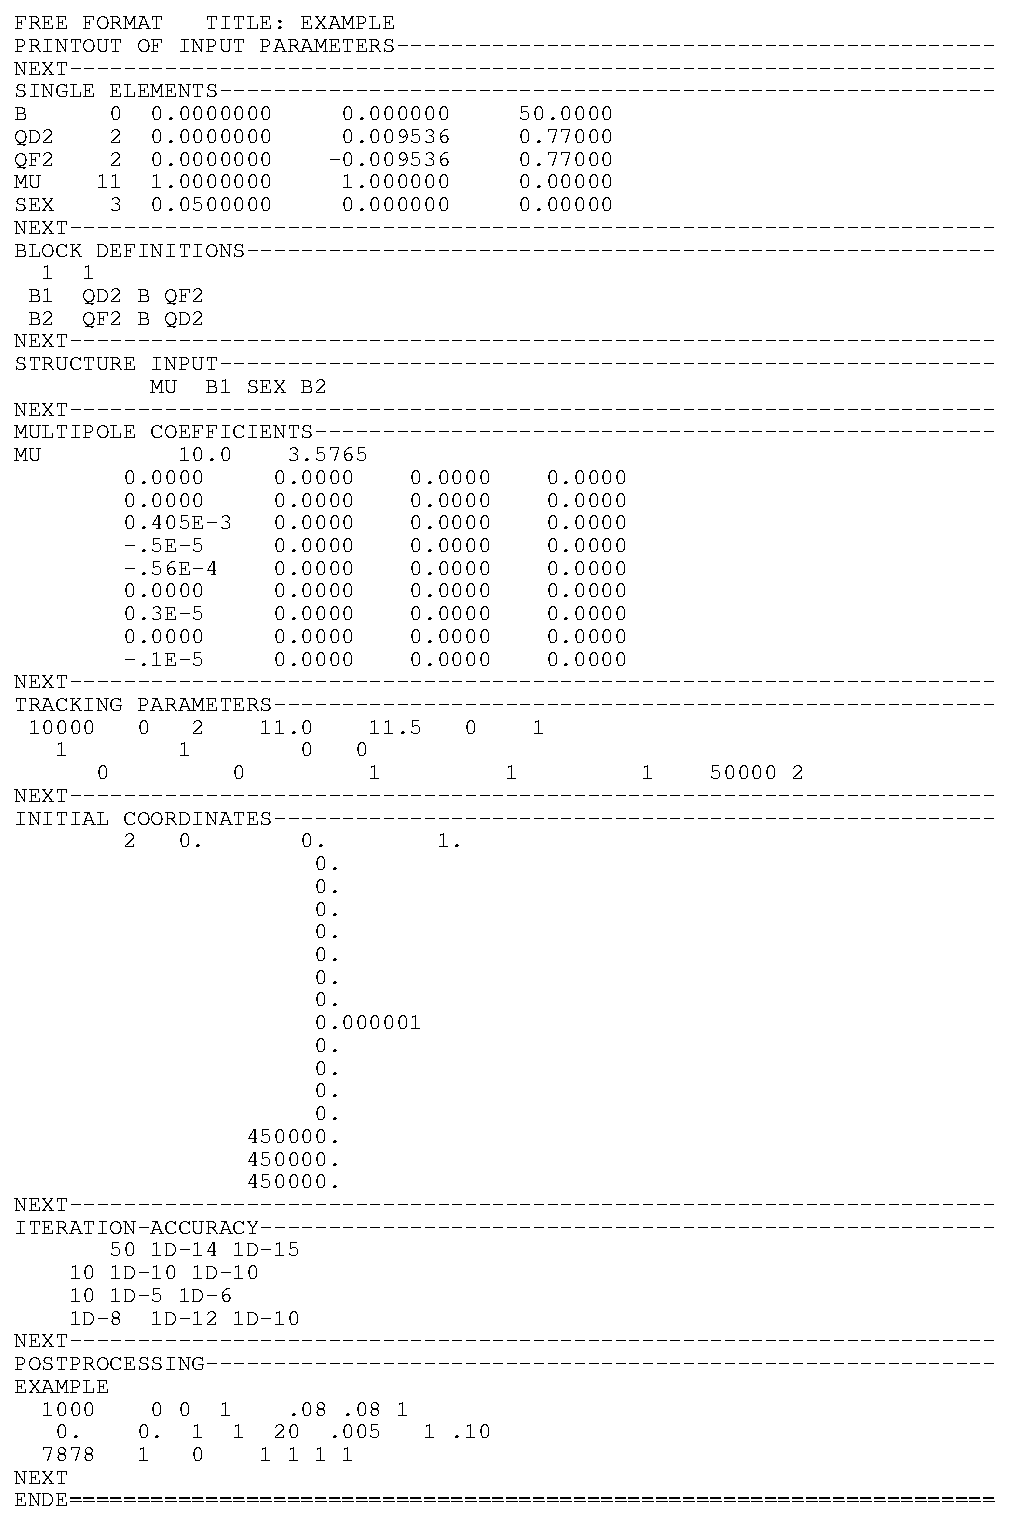
\includegraphics[height=14cm]{figures/expout1}
%     \end{center}
% \end{figure}

\clearpage

% ================================================================================================================================ %
\section{Output Example} \label{output}

The preprocessing part is shown first.

\begin{ctverbatim}
-----------------------------------------------------------------------------------------------------------------------------------

    OOOOOOOOOOOOOOOOOOOOO
    OO                 OO
    OO  PREPROCESSING  OO
    OO                 OO
    OOOOOOOOOOOOOOOOOOOOO

-----------------------------------------------------------------------------------------------------------------------------------


    STRUCTURE INPUT FILE HAS -THICK- LINEAR ELEMENTS


---- ENTRY CLORB ----/DPP= 0.00000 /CLOX/   0.00000   0.00000 /CLOY/   0.00000   0.00000 /ITERAT.=  2/ ACCURACY= 0.000000D+00
---- ENTRY CLORB ----/DPP= 0.00000 /CLOX/   0.00000   0.00000 /CLOY/   0.00000   0.00000 /ITERAT.=  2/ ACCURACY= 0.000000D+00
---- ENTRY CLORB ----/DPP= 0.00000 /CLOX/   0.00000   0.00000 /CLOY/   0.00000   0.00000 /ITERAT.=  2/ ACCURACY= 0.000000D+00
---- ENTRY CLORB ----/DPP= 0.00000 /CLOX/   0.00000   0.00000 /CLOY/   0.00000   0.00000 /ITERAT.=  2/ ACCURACY= 0.000000D+00

    Initial 4-D DA CLOSED ORBIT IN QMODDA (NO TUNE ADJUSTEMENT)
        0.000000000000000000000000000000000
        0.000000000000000000000000000000000
        0.000000000000000000000000000000000
        0.000000000000000000000000000000000

-----------------------------------------------------------------------------------------------------------------------------------
     DA INITIALIZATION: ORDER =  1, # of VARIABLES =  4, DIMENSION =  2


-----------------------------------------------------------------------------------------------------------------------------------
    ENTERING 4-D DA CLOSED ORBIT CALCULATION

---- closed orbit before correction----
 CLOX    0.00000000       0.00000000    
 CLOY    0.00000000       0.00000000    
---- after DA correction----
 CLOX    0.00000000       0.00000000    
 CLOY    0.00000000       0.00000000    
 ITERAT.=  1 ACCURACY= 0.000000D+00

SUCCESSFULL END OF 4-D DA CLOSED ORBIT CALCULATION IN ITERATION:    1

 CLOX    0.00000000       0.00000000    
  D-X    0.00000000       0.00000000    
 CLOY    0.00000000       0.00000000    
  D-Y    0.00000000       0.00000000    
 ITERAT.=  1 ACCURACY= 0.000000D+00


-----------------------------------------------------------------------------------------------------------------------------------
     DA INITIALIZATION: ORDER =  2, # of VARIABLES =  4, DIMENSION =  2

Check of the symplectic condition on the linear part
0.000000000000000       0.9999999999999998        0.000000000000000        0.000000000000000    
-0.9999999999999998        0.000000000000000        0.000000000000000        0.000000000000000    
0.000000000000000        0.000000000000000        0.000000000000000       0.9999999999999996    
0.000000000000000        0.000000000000000      -0.9999999999999996        0.000000000000000    
deviation for symplecticity   -3.3306690738754709E-014  %
0.12223867786724546       0.12223867786724549     

-----------------------------------------------------------------------------------------------------------------------------------

    TRACKING FOR CONSTANT MOMENTUM DEVIATION

          ------ NO ACCELERATION ------

                TUNE         CLO            CLOP              BET0           ALF0           GAMMA      

      X    0.1222386779   0.0000000       0.0000000        92.957545511    0.0000000000    0.010757599
                                                            0.000000000   -0.0000000000    0.000000000
      Y    0.1222386779   0.0000000       0.0000000       203.581213058   -0.0000000000    0.004912045
                                                            0.000000000   -0.0000000000    0.000000000


    REL. MOMENTUM DEVIATION= 0.0000000000000000
  ========================================

---- CLOSED ORBIT AND DECOUPLING (1=COU,0=DECOU)
/CLX /            0.000000000000000000000000000000000
/CLXP/            0.000000000000000000000000000000000
/CLY /            0.000000000000000000000000000000000
/CLYP/            0.000000000000000000000000000000000
/DCX /    1
/DCY /    1env
env
/IVER /   0
/IDFOR/   0
/ICLO6/   0
/ITION/   0
\end{ctverbatim}

% \begin{figure}[H]
% \begin{center}
%     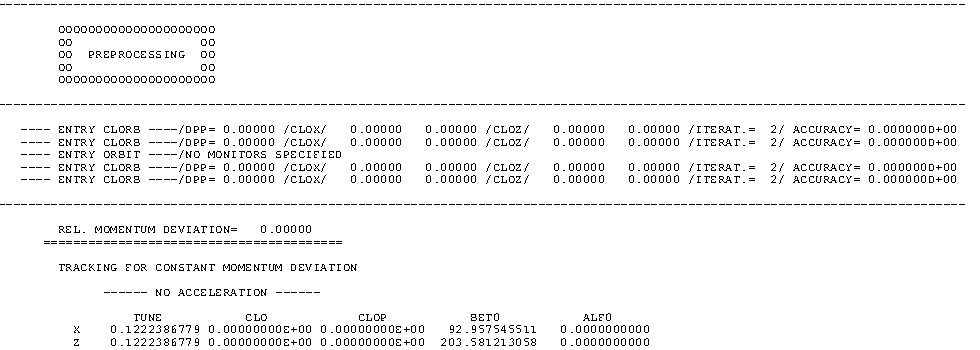
\includegraphics[width=16cm,height=13cm]{figures/expout2}
% \end{center}
% \end{figure}

\clearpage

Followed by the initial coordinates.

\begin{ctverbatim}
-----------------------------------------------------------------------------------------------------------------------------------

         OOOOOOOOOOOOOOOOOOOOOOOOOOO
         OO                       OO
         OO  INITIAL COORDINATES  OO
         OO                       OO
         OOOOOOOOOOOOOOOOOOOOOOOOOOO

-----------------------------------------------------------------------------------------------------------------------------------



     PARTICLE       3 RANDOM SEED        0 MOMENTUM DEVIATION   0.0000    


     ---- TWIN-TRAJECTORIES NO CL.ORBIT ADDED
     /X1  /           11.500000000000000000000000000000000
     /XP1 /           -0.000000000000000019769953827468216
     /Y1  /           17.018620942597696199527490534819663
     /YP1 /            0.000000000000000000000000000000000
     /SIG1/            0.000000000000000000000000000000000
     /DP1 /            0.000000000000000000000000000000000
     /X2  /           11.500000000000000000000000000000000
     /XP2 /            0.000000999999999980229994000959642
     /Y2  /           17.018620942597696199527490534819663
     /YP2 /            0.000000000000000000000000000000000
     /SIG2/            0.000000000000000000000000000000000
     /DP2 /            0.000000000000000000000000000000000


         UNCOUPLED AMPLITUDES AND EMITTANCES:
         AMPLITUDE-X =          11.500          AMPLITUDE-Y =          17.019  MM
         EMITTANCE-X =           1.423          EMITTANCE-Y =           1.423  PI*MRAD*MM

     ---- INITIAL COORD. OF TWIN-TRAJECTORIES
                     11.500000000000000000000000000000000
                     -0.000000000000000019769953827468216
                     17.018620942597696199527490534819663
                      0.000000000000000000000000000000000
                      0.000000000000000000000000000000000
                      0.000000000000000000000000000000000
                     11.500000000000000000000000000000000
                      0.000000999999999980229994000959642
                     17.018620942597696199527490534819663
                      0.000000000000000000000000000000000
                      0.000000000000000000000000000000000
                      0.000000000000000000000000000000000
                 450000.000000000000000000000000000000000
                 449999.999999999941792339086532592773438
                 449999.999999999941792339086532592773438

 
------------------------------------------------------------------------------------------------------------------------------------
 
  CALL TO CADCUM
 
 Machine length was    103.0800000000 [m]
\end{ctverbatim}

\clearpage

And the final coordinates for a regular (right side) and chaotic (left side) case.

\begin{ctverbatim}
-----------------------------------------------------------------------------------------------------------------------------------

         OOOOOOOOOOOOOOOO
         OO            OO
         OO  TRACKING  OO
         OO            OO
         OOOOOOOOOOOOOOOO

-----------------------------------------------------------------------------------------------------------------------------------


 
 Calling thck4d subroutine
 

     PARTICLE       1 AND       2 STABLE - RANDOM SEED        0 MOMENTUM DEVIATION   0.0000    
     REVOLUTION    10000

                      6.413505260046698630560513265663758
                     -0.089292907574702679029954310863104
                     -6.601359435036310507882717502070591
                      0.081356939205201914133702700837603
                      0.000000000000000000000000000000000
                      0.000000000000000000000000000000000
                      6.407742554197603190857535082614049
                     -0.089306143545032981578835062919097
                     -6.608681191308765967562521836953238
                      0.081353966356037088480945840274217
                      0.000000000000000000000000000000000
                      0.000000000000000000000000000000000
                 450000.000000000000000000000000000000000
                 449999.999999999941792339086532592773438
                 449999.999999999941792339086532592773438

     PARTICLE       3 AND       4 STABLE - RANDOM SEED        0 MOMENTUM DEVIATION   0.0000    
     REVOLUTION    10000

                     11.004259035154733581407526799011976
                     -0.017944489717545052120950543894651
                    -17.049149437508784643569015315733850
                      0.015505328739040841190544028904696
                      0.000000000000000000000000000000000
                      0.000000000000000000000000000000000
                     10.717352036206978738164252717979252
                     -0.079677127850136961195737228536018
                      5.973322092980881237167523067910224
                     -0.075407170859343758406723168263852
                      0.000000000000000000000000000000000
                      0.000000000000000000000000000000000
                 450000.000000000000000000000000000000000
                 449999.999999999941792339086532592773438
                 449999.999999999941792339086532592773438

-----------------------------------------------------------------------------------------------------------------------------------
\end{ctverbatim}

% \begin{figure}[H]
% \begin{center}
%     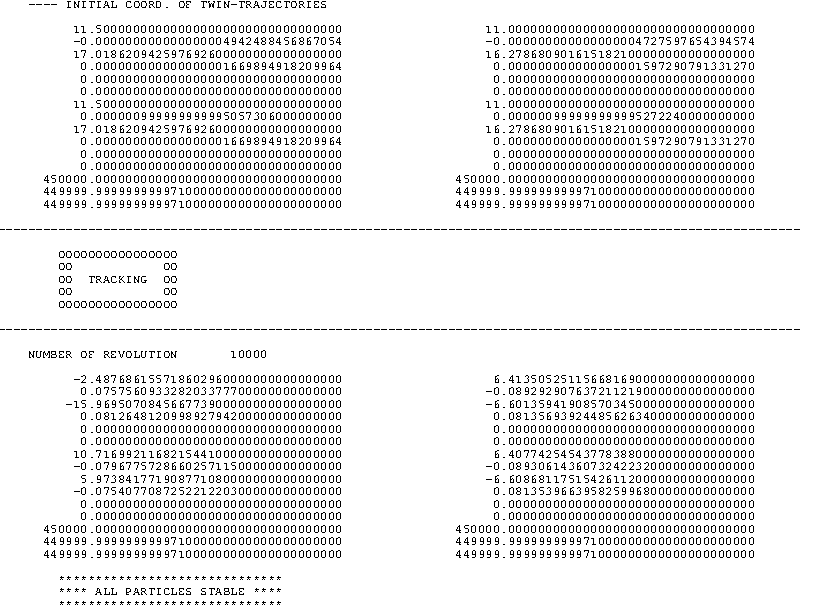
\includegraphics[width=16cm,height=13cm]{figures/expout3}
% \end{center}
% \end{figure}

\clearpage

Finally part of the post--processing for the two particle pairs are shown (chaotic on the left and regular on the right respectively) and a summary of the post--processing is given.

\begin{ctverbatim}

\end{ctverbatim}

% \begin{figure}[H]
% \begin{center}
%   \mbox{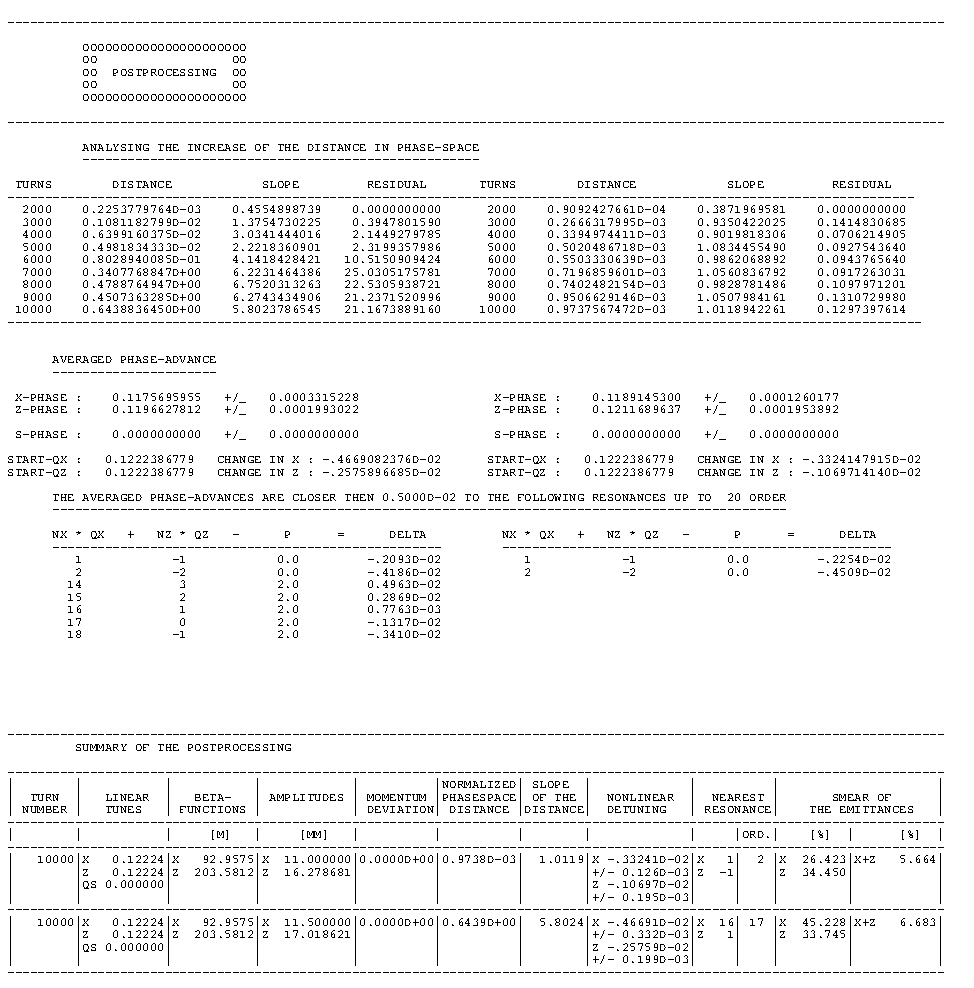
\includegraphics[width=16cm,height=21cm]{figures/expout4}}
% \end{center}
% \end{figure}

\clearpage

\section{Plot Example} \label{plots}

{\small In figure~\ref{Lya} a typical example of the evolution of the
  distance in phase space is shown of a regular and chaotic particle.
  Figure~\ref{H-proj} and figure~\ref{P-proj} show the corresponding
  horizontal phase space and the physical phase space projections
  respectively. An example of the stroboscoped phase space is shown in
  figure~\ref{P-stro}, where the motion in the chaotic case is beyond
  a ``separatrix'' in the four--dimensional phase space. Even in the
  FFT (figure~\ref{P-FFT}) one can see the effect of chaotic
  behaviour: it leads to a widening of the lines of the spectrum.}
\begin{figure}[H] \vspace*{-5mm}
\begin{center}
  \mbox{\includegraphics*[width=9.cm]{figures/exp1}}
  \\[5mm]
  \mbox{\includegraphics*[width=9.cm]{figures/exp9}}
 \caption{\small Evolution of the Distance of Phase Space for Regular
   \mbox{(upper part)} and Chaotic \mbox{(lower part)} Motion.}
 \label{Lya}
\end{center}
\end{figure} 

\begin{figure}[H]
\begin{center}
  \mbox{\includegraphics*[width=10.5cm]{figures/exp2}}
  \\[5mm]
  \mbox{\includegraphics*[width=10.5cm]{figures/exp10}}
 \caption{Horizontal Phase Space Projections for the
   Regular (upper part) and the Chaotic \mbox{(lower part)} Cases.}
 \label{H-proj}
\end{center}
\end{figure}

\begin{figure}[H]
\begin{center}
  \mbox{\includegraphics*[width=10.5cm]{figures/exp4}}
  \\[5mm]
  \mbox{\includegraphics*[width=10.5cm]{figures/exp12}}
 \caption{Physical Phase Space Projections for the Regular
   \mbox{(upper part)} and the Chaotic \mbox{(lower part)} Cases.}
 \label{P-proj}
\end{center}
\end{figure}

\begin{figure}[H]
\begin{center}
  \mbox{\includegraphics*[width=10.5cm]{figures/exp6}}
  \\[5mm]
  \mbox{\includegraphics*[width=10.5cm]{figures/exp14}}
 \caption{\small{Stroboscoped Vertical Phase Space Projections
     for the Regular (upper part) and the Chaotic (lower part) Cases
     respectively.  The regular motion stays inside a ``separatrix''
     with two unstable fix--points visible, while the chaotic motion
     is clearly outside this ``separatrix''.}}
 \label{P-stro}
\end{center}
\end{figure}

\begin{figure}[H]
\begin{center}
  \mbox{\includegraphics*[width=10.5cm]{figures/exp7}}
  \\[5mm]
  \mbox{\includegraphics*[width=10.5cm]{figures/exp15}}
 \caption{Horizontal FFT--Analysis for the Regular (upper part)
   and the Chaotic (lower part) Cases.}
 \label{P-FFT}
\end{center}
\end{figure}
